\subsection{CU8 Visualizar Refacciones Disponibles}
Regresando un poco a la pantalla de Visualización del Menú (figura \ref{fig:Pantalla Visualizar Menu - Vista de Escenarios}), al pulsar el botón de 'Gestionar las Refacciones', aparece esta pantalla. Muy simular a la visualización de los registros pero aquí el usuario solamente podrá ver y buscar las refacciones que hay en existencia en el almacén del taller. En caso de que no exista alguno, podrá presionar el botón de la parte inferior 'Solicitar Refacción'.
\\
En la tabla el usuario podrá observar los registros a manera de lista dentro de una tabla, con los campos: Num. de Solicitud, una Descripción, la Fecha de Solicitud y la Existencia en almacén. 
\\
Al presionar el botón de salir, el sistema cerrará esta pantalla y regresará a la Visualización del Menú. 
\begin{figure}[!h]
	\centering
	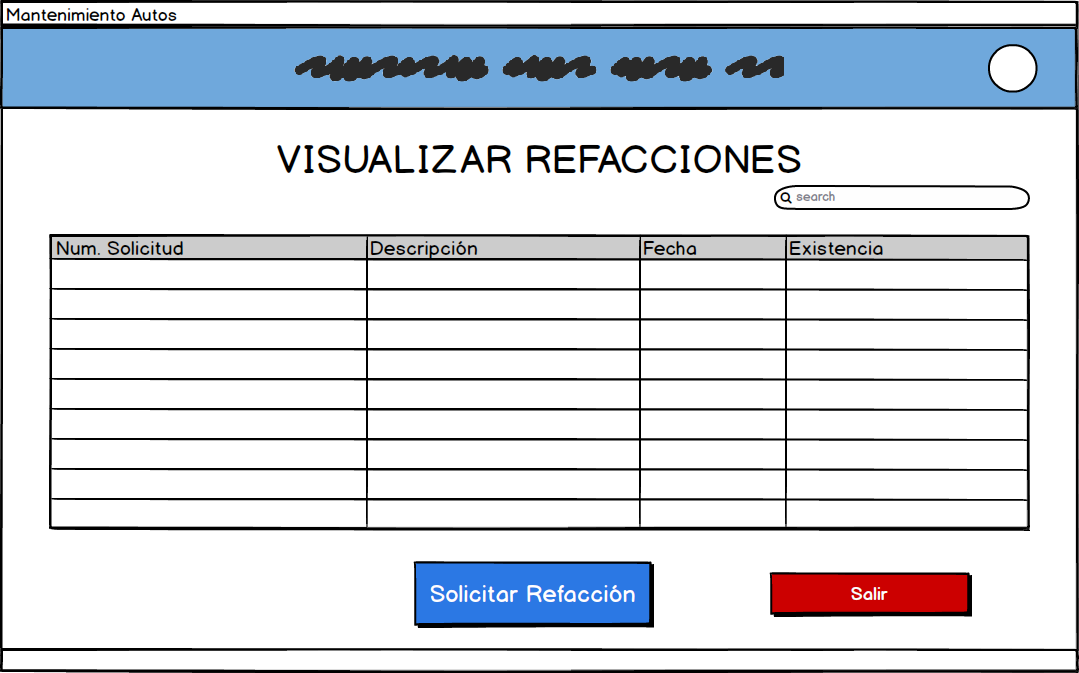
\includegraphics[width=1\textwidth]{./diseno/vescenarios/imagenes/VisualizarRefacciones}
	\caption{Pantalla Visualizar Refacciones - Vista de Escenarios}
	\label{fig:Pantalla Visualizar Refaccioes - Vista de Escenarios}
\end{figure}
\clearpage